\documentclass[a4paper,12pt]{article}
\usepackage{geometry}
\usepackage[english]{babel}
\usepackage[utf8]{inputenc}
\usepackage{amsmath,amssymb,mathabx}%\for eqref
\usepackage{xcolor}
%\usepackage{fancyhdr}
\usepackage{url}
\usepackage{tikz}
%\usepackage[backend=biber,autocite=plain,backref=true]{biblatex}
%\usepackage[backend=biber,hyperref,autocite=plain,backref=true]{biblatex}
%\usepackage[backend=biber,sorting=none,autocite=plain,backref=true]{biblatex}
\usepackage[backend=biber,style=alphabetic]{biblatex}
%\usepackage[backend=biber,style=numeric,autocite=superscript,sorting=none]{biblatex}

\addbibresource{lecture1claude.bib}
\addbibresource{claude.bib}

\title{The Institute for Advanced Study \\ Group Theory and Spectroscopy }
\author{Giulio Racah \\The Hebrew University, Jerusalem\\Notes by Eugen Merzbacher and David Park}
\date{Spring, 1951}

\begin{document}
\maketitle
\section*{Preface}
These notes are based on a series of seminar lectures given during the 1951
Spring term at the Institute for Advanced Study. Owing to limitations of time
only particular topics were considered, and there is no claim to completeness.
Since it is intended to publish later a more complete treatment of the subject,
comments about these notes as well as suggestions concerning the desirability
of adding related topics will be appreciated and should be addressed to the
author at the Hebrew University, Jerusalem, Israel.

As the limited supply of these notes makes it impossible to send more than one
cony to any institution, it is requested that all copies be made available to
departmental libraries.

Also known as G. Racah, Group Theory and Spectroscopy, Report CERN61-8 (CERN, Geneva, 1961).
\tableofcontents


\begin{enumerate}
\setcounter{enumi}{2}
\item THE REPRESENTATIONS OF THE SEMI-SIMPLE GROUPS
\begin{enumerate}
\item 32 Representations and weights
\item 37 The classification of the irreducible representations
\item 42 The problem of full reducibility
\item 44 Casimir's operator and its generalization
\item 50 Miscellaneous problems
\item 55 The full linear group and the unitary group
\end{enumerate}
\item THE EIGENFUNCTIONS OF THE NUCLEAR SHELLS
\begin{enumerate}
\item 1. Introduction ..... 57
\item 2. The coefficients of fractional parentage ..... 58
\item 3. The classification of the states \(\ell^n\) ..... 62
\item 4. The factorization of the coefficients of fractional parentage ..... 66
\item 5. The algebra of tensor operators ..... 69
\item 57 Tensor operators and Lie groups
\item 78 Calculation of the coefficients of fractional parentage
\end{enumerate}
\item THE CALCULATION OF THE ENERGY MATRIX
\begin{enumerate}
\item 89 The interaction of two particles
\item 90 The group-theoretical classification of the interactions
\item 97 Calculation of the energy matrices
\item 101 Spin-dependent interactions
\end{enumerate}
\end{enumerate}

These lectures will treat the applications of group theory to problems of
spectroscopy and nuclear structure. While developing the mathematical tools for
this purpose, we shall occasionally forego the elaboration of a rigorous proof.
In such cases, references will be quoted.

\textcolor{red}{My corrections} \textcolor{blue}{and my calculations needed to
follow the discussion are set off by colored text. DMD}

\section{General Notions on Continuous Groups}
``We shall therefore from this point on restrict ourselves to the study of semi-simple groups.'' 
\subsection{Continuous groups and infinitesimal groups}
%\section{General Notions on Continuous Groups}
%\subsection{Continuous Groups and Infinitesimal Groups}

We start with a set of \(n\) variables \(x_0^i\), \(i=1 \ldots n\), which may be
regarded as coordinates of a point in a certain space. Consider now the set of equations
\begin{equation}\label{eq:1}
x^i=f^i\left(x_0^1, \ldots, x_0^n ; a^1, \ldots, a^r\right) \quad(i=1 \ldots n),
\end{equation}
in which the \(a^\rho\) appear as a set of \(r\) independent parameters.
Omitting indices, we shall write this and similar relations in the form
\[
x=f\left(x_0 ; a\right) \quad \text { or } \quad x=S_a x_0 \tag{1'}
\]

These equations define a set \(S\) of transformations, depending on the
parameters \(a\), which map the point \(x_0\) onto \(x\). We shall assume
that the \(f^i\) have all the required derivatives, and that the \(f^i\) depend
\underline{essentially}
on the parameters, i.e., that no two transformations with different
parameters are the same for all values of \(x_0\), so that \(r\) is the
smallest number of parameters needed to specify the transformations completely
and uniquely.


The set of transformations \(f\) is said to form a group if it obeys the
following two conditions:
\begin{itemize}
\item [i)]
The result of performing successively any two transformations of the set is
another transformation belonging to this set. Formally, if
\(x=f\left(x_0 ; a\right)\) and \(x^{\prime}=f(x ; b)\)
then there exists a set of parameters \(c^\rho\)
\begin{equation}\label{eq:2}
c^\rho=\varphi^\rho(a ; b)
\end{equation}
such that
\begin{equation}\label{eq:3}
x^{\prime}=f(x ; b)=f\left(f(x_0; a) ; b\right)=f(x_0 ; c)=f(x_0 ; \varphi(a ; b)).
\end{equation}
\item [ii)]
Corresponding to every transformation there exists a unique inverse, which also
belongs to the set: Given equation (\ref{eq:1}) there exists a set of
parameters \(\bar{a}\) such that \(x_0=f(x ;\bar{a})\).
\end{itemize}

The uniqueness of \(\bar{a}\) is guaranteed if the Jacobian of the transformation does not vanish:
\begin{equation}\label{eq:4}
\left|\frac{\partial f}{\partial x_0}\right| \neq 0
\end{equation}

Transforming \(x_0\) onto \(x\) and then inversely \(x\) back to \(x_0\), we
obtain according to i) a transformation which belongs to the group and is
characterized by the set of parameters \(a_0\). Since the transformation
depends on the parameters in an essential way, the \(a\) so constructed cannot
depend on the particular value of the parameters from which we started. The
transformation \(f(x, a_0)\) is called the identity.

Since it imposes no restriction, we shall take:
\[
a_0^\rho=\textcolor{red}{0} \quad (\rho=1 \ldots r). \quad 
\]
\(r\) is called the \underline{order} of the group. (Note that this usage is
different from that found in the theory of finite groups.)

We also remind the reader of the following definitions: A mapping of one group
onto another is said to be \underline{homomorphic} or a
\underline{homomorphism} if it preserves the operation of group multiplication.
We call such a mapping an \underline{isomorphism} if, in addition, the
correspondence between elements of the two groups is one-to-one.  Since the
combination law of the transformations (\ref{eq:1}) is given in terms of the
parameters \(a\), there can be transformations corresponding to different
values of \(n\) which are homomorphic or even isomorphic.

A group of linear transformations which is homomorphic with a given group is called a
\underline{representation} of this group.

The fundamental idea of Sophus Lie's theory of continuous groups~\cite{Lie1893} is to consider
not the whole of a group, but that part of it which lies near the identity,
consisting of the so-called \underline{infinitesimal}
\underline{transformations}. Thus, instead of the finite displacement of a
point under a transformation, we consider the application of successive
infinitesimal displacements - we think of a generalized velocity field
describing the motion of a point from its original position \(x_0\) to its
final position \(x\).
\textcolor{blue}{The velocity field is independent of the parameters.}


We have now two equivalent expressions for x:
\begin{subequations}\label{eq:5}
  \begin{align}
x=f(x_0; a), \label{eq:5a} \\
x=f(x; 0).  \label{eq:5b}
  \end{align}
\end{subequations}
Corresponding to these we can represent in either of two ways a transformation,
as a result of which the new components of \(x\) differ infinitesimally from
the old ones - by differentiation of (\ref{eq:5a}) or by introducing a parameter
of infinitesimal size in (5b):
\[
x+d x=f\left(x_0 ; a+d a\right) \quad \text{or} \quad
x+d x=f\left(x; \delta a\right)
\]
or (employing the summation convention),
\begin{equation}\label{eq:6}
d x=\frac{\partial f\left(x_{0}; a\right)}{\partial a^\sigma} d{a}^\sigma
\quad \text{or} \quad
d x=\left(\frac{\partial f(x ; a)}{\partial a^\sigma}\right)_{a=0} \delta a^\sigma.
\end{equation}
The last may be written
\begin{equation}\label{eq:7}
d x^i=u_\sigma^i(x) \delta a^\sigma, \quad
u_\sigma^i(x)=\left(\frac{\partial f^i(x; a)}{\partial a^\sigma}\right)_{a=0}
\end{equation}
which defines the ``velocity field'' \(u_\sigma^i(x)\) mentioned above.
\textcolor{blue}{The velocity field is independent of the parameters.}
In the notation of (\ref{eq:2}) we may write
\[
a+d a=\varphi(a ; \delta a) .
\]
Since it follows from (\ref{eq:2}) and (\ref{eq:5}) that \(\varphi(a ; 0)=a\), we have
\[
a+d a=a+\left(\frac{\partial \varphi(a ; b)}{\partial b^\tau}\right)_{b=0} \delta a^\tau .
\]
Thus, da is a linear combination of \(\delta a\) :
\begin{equation}\label{eq:8}
d a^\rho=\mu_\tau^\rho(a) \delta a^\tau, \quad \mu_\tau^\rho(a)=
\left(\frac{\partial \varphi^\rho(a; b)}{\partial b^{\tau}}\right)_{b=0}
\end{equation}

Solving for \(\delta a\), we get
\[
\delta a^\sigma=\lambda_{\rho}^{\sigma} (a) ~~ d {a}^{\rho} \tag{8'}
\]
where
\begin{equation}\label{eq:9}
\lambda \mu=1, \qquad \text{i.e.}~~
\lambda_{\rho}^\sigma \mu_\tau^\rho=\delta_\tau^\sigma.
\end{equation}
From (6), (7) and (8') we get the first fundamental formula:
\[
\frac{\partial x^i}{\partial a^{\rho}} = u^i_{\tau}(x) \lambda^{\tau}_{\rho} (a) \tag{A}
\]
If \(u\) is to represent the velocity field of a transformation (\ref{eq:1}), equation
(A) must be completely integrable, i.e. it must be capable of admitting
solutions with \(n\) arbitrary constants \(x_0\). The integrability condition
\[
\frac{\partial^2 x^i}{\partial a^{\sigma} \partial a^{\rho}}=
\frac{\partial^2 x^i}{\partial a^{\rho} \partial a^{\sigma}}
\]
\textcolor{blue}{
\[
\frac{\partial^2 x^i}{\partial a^{\sigma} \partial a^{\rho}}=
\left( \frac{\partial}{\partial a^{\sigma}} u^i_{\nu} \right) \lambda^{\nu}_{\rho}+
u^i_{\nu} \frac{\partial \lambda^{\nu}_{\rho}}{\partial a^{\sigma}} 
\]
\[
\frac{\partial u^i_{\nu} }{\partial a^{\sigma}}  =
\frac{\partial u^i_{\nu} }{\partial x^{j}} 
\frac{\partial x^{j}}{\partial a^{\sigma}}, \quad
\frac{\partial x^j}{\partial a^{\sigma}} = 
u^j_{\tau} \lambda^{\tau}_{\sigma}
\]
\[
\frac{\partial u^i_{\nu} }{\partial a^{\sigma}} \lambda^{\nu}_{\rho}=
\frac{\partial u^i_{\nu} }{\partial x^{j}} 
u^j_{\tau} \lambda^{\tau}_{\sigma}
 \lambda^{\nu}_{\rho}
\]
}
becomes
\textcolor{red}{
\[
\left( u_{\kappa}^j \frac{\partial u^i_{\nu}}{\partial x^j}-
u^j_{\nu} \frac{\partial u_{\kappa}^i}{\partial x^j}\right)
\lambda_{\sigma}^{\kappa} \lambda^{\nu}_{\rho} +
u^i_{\nu} \left( \frac{\partial \lambda_\sigma^\nu}{\partial a^{\rho}}-
\frac{\partial \lambda_{\rho}^{\nu}}{\partial a^{\sigma}} \right)=0.
\]
}
and, using (\ref{eq:9}),
\textcolor{blue}{
\[
d_{\kappa \nu}^{i} := 
u_{\kappa}^j \frac{\partial u^i_{\nu}}{\partial x^j}-
u^j_{\nu} \frac{\partial u_{\kappa}^i}{\partial x^j}, \quad
e^{\tau}_{\rho  \sigma} := 
\frac{\partial \lambda_{\rho}^{\nu}}{\partial a^{\sigma}} -
 \frac{\partial \lambda_\sigma^\nu}{\partial a^{\rho}}
\]
\[
\lambda^{\nu}_{\rho} \mu^{\rho}_{q} =\delta^{\nu}_{q}, \quad
\lambda^{\kappa}_{\sigma} \mu^{\sigma}_{m} =\delta^{\kappa}_{m}, \quad
d_{\kappa \nu}^{i} \lambda_{\sigma}^{\kappa}
\lambda^{\nu}_{\rho} \mu^{\sigma}_{m} \mu^{\rho}_{q} = d_{q m}^{i} =
u^i_{\tau} e^{\tau}_{\rho  \sigma} \mu^{\sigma}_{m} \mu^{\rho}_{q} 
\]
}
this gives \textcolor{blue}{equation B1,}
\begin{equation}\label{eq:10}
u_{\kappa}^j \frac{\partial u^i_{\nu}}{\partial x^j}-
u^j_{\nu} \frac{\partial u_{\kappa}^i}{\partial x^j} =
c_{\kappa \nu}^{\tau}(a)  u_{\tau}^{i}
\end{equation}
where
\begin{equation}\label{eq:11}
c_{\kappa \nu}^{\tau}(a) = \left(
\frac{\partial \lambda^{\tau}_{\rho}}{\partial a^{^\sigma}}-
\frac{\partial \lambda_{\sigma}^{\tau}}{\partial a^\rho}
\right)
\mu_{\kappa}^\rho \mu_{\nu}^{\sigma}.
\end{equation}
Since \(u\) is independent of \(a\), differentiation of (10) by \(a^{\rho}\) gives
\[
\frac{\partial c_{x \nu}^\tau(a)}{\partial a^{\rho}} u_\tau^i=0 .
\]
But the a's have been assumed essential, so that by (7) the u's are
linearly independent, hence the c's are independent of \(a\).  From (\ref{eq:11})
\[
\frac{\partial \lambda_{\rho}^{\tau}}{\partial a^{\sigma}} -
 \frac{\partial \lambda_\sigma^\tau}{\partial a^{\rho}} =
c_{\kappa \nu}^{\tau} \lambda_\rho^{\kappa} \lambda_\sigma^\nu. \tag{B2}
\]
(B1) is a necessary condition on the velocity field if the latter is to
generate a group, and (B2) is a corresponding restriction on the manner in which
the a's combine.

An infinitesimal transformation on the \(x\) induces on any function \(F(x)\) a variation
\begin{equation}\label{eq:12}
d F(x)=\frac{\partial F}{\partial x^i} d x^i=
\delta a^\sigma u_\sigma^i \frac{\partial F}{\partial x^i} \equiv \delta a^\sigma x_\sigma F
\end{equation}
where
\begin{equation}\label{eq:13}
x_\sigma=u_\sigma^i(x) \frac{\partial}{\partial x^i}
\end{equation}
(\ref{eq:12}) shows that every infinitesimal transformation of \(F(x)\) is generated by
a linear combination of the operators \(X\) which are called the infinitesimal
operators of the group \(S\). From \(\left(B_1\right)\) it follows that they
satisfy the relation
\begin{equation}\label{eq:14}
x_\rho x_\sigma-x_\sigma x_\rho \equiv\left[x_\rho x_\sigma\right]=c_{\rho \sigma}^\tau x_\tau .
\end{equation}
Evidently
\[
c_{\rho \sigma}{ }^\tau=-c_{\sigma \rho}{ }^\tau .
\tag{C1}
\]
Substituting (14) into the Jacobi identity
\[
\left[\left[X_\rho X_\sigma\right] X_\tau\right]+
\left[\left[X_\sigma X_\tau\right] X_\rho\right]+
\left[\left[X_\tau X_\rho\right] X_\sigma\right]=0
\]
we get
\[
c_{p \sigma}{ }^\mu c_{\mu \tau}{ }^\nu+c_{\sigma \tau}^\mu c_{\mu p}^\nu+c_{\tau \rho}{ }^\mu c_{\mu \sigma}{ }^\nu=0.
\tag{C2}
\]
We have shown that equations (c) are implied if the \(f^i\) form a group. That the converse to this statement holds is the content of the three fundamental theorems of Lie~\cite{Lie1893}, which we shall not prove. They state that
\begin{itemize}
\item[I.] If there exist \(f^i=x^i\) satisfying (A) then they form a group.
\item[II.] If there exist u's satisfying \(\left(B_1\right)\), then there exist \(\lambda\) 's, determined within isomorphism, which satisfy \(\left(B_2\right)\), so that equation (A) is integrable.
\item[III.] For every set of o's satisfying (C), there exist u's satisfying \(\left(B_1\right)\).
\end{itemize}
We shall write an infinitesimal transformation of the group \(S\) in the form
\[
S_a=1+\delta a^\sigma X_\sigma,
\]
where \(\delta a^\sigma\) is an infinitesimal quantity defined to be of
the first order. If we combine two such transformations, we get
\[
S_a S_b= \left(1+\delta a^{\rho} X_\rho\right)\left(1+\delta a^{\sigma} X_{\sigma}\right)=
1+\delta a^{\rho} X_{\rho}+\delta a^{\sigma} X_{\sigma},
\]
where the first non-vanishing infinitesimal terms have been retained.
Thus, to the operation of multiplication in \(S\) corresponds addition in the
infinitesimal group of \(S\). If the first order quantities vanish, we have to
consider quantities of higher order. But the second theorem of Lie implies that
in this connection we need never go beyond the second order of infinitesimals -
i.e. we have only to worry about commutators, which are expressions of the form
\(S_a S_b S_a^{-1} S_b^{-1}\), and to ask that the corresponding infinitesimal
operator of the second order,
\[\delta a^{\rho} \delta b^\sigma\left[X_\rho X_\sigma\right]
\]
be contained in the linear manifold of infinitesimal operators.

\subsection{Parameter Groups and Adjoint Groups}
%\section{Parameter Groups and Adjoint Groups.}
On comparing (8) with (7), we see that a close formal analogy exists between
the functions \(\mu\) and \(u_0\) In fact, the \(\varphi(a, b)\) of (2) which
connect the parameters according to the composition law of the group may
themselves be considered as defining a group in the same way as does (1'),
\[
{a^{\prime}}^{\rho}=\varphi^{\rho}(a ; b)
\]
This relation can be regarded as a mapping of the a onto the a' according to a
transformation whose parameter is b. We shall prove that these transformations
form a group \(P_1\), which is isomorphic with \(S\) and is called the \underline{first}
\underline{parameter} \underline{group}. Indeed, if \(a=\varphi(a ; b)\) and \(a^{\prime
\prime}=\varphi(a ; ; c)\) then
\[
a^{\prime \prime}=\varphi(\varphi(a ; b) ; c)=\varphi(a ; \varphi(b ; c))
\]
where the last equality follows from the associative property of the
transformations \(f^i\). We thus see that the law of composition is the same
for the first parameter group and the original group of transformations \(f^i\).

The analogous group of transformations on the argument \(b\) of \(\varphi(a ;
b)\) is called the \underline{second} \underline{parameter} \underline{group}
second paramete\(P_2\). \(P_2\) is anti-isomorphic with \(S\),
that is, it is isomorphic when the factors are taken in the reverse
order. But since \((x y)^{-1}=y^{-1} x^{-1}\) and since a group contains
\(x^{-1}\) if it contains \(x\), the two are in fact isomorphic. Let a (or c)
be a transformation belonging to the first (or second) parameter group. Let the
operation of \(P_1\) transform \(b\) into \(b:=\varphi(b, a)\) and let the
operation of \(P_2\) transform \(b^{\prime}\) into
\(b^{\prime \prime}=\varphi\left(c, b^{\prime}\right)\). Then it is clear that
\[
b^{\prime \prime}=\varphi\left(c, b^{\prime}\right)=
\varphi(c, \varphi(b, a))=\varphi(\varphi(c, b), a),
\]
hence every element of \(P_1\) commutes with every element of \(P_2\).
The \(\mu^{\prime} s\) are the velocity field of \(P_1\) (see equation (\ref{eq:8})),
and they define the infinitesimal operator
\begin{equation}\label{eq:15}
A_\tau=\mu_\tau^{\rho} (a) \frac{\partial}{\partial a^{\rho}} .
\end{equation}
Correspondingly, in \(\mathrm{P}_2\)
\begin{equation}\label{eq:16}
B_\tau={\overline{\mu}}^{\rho}_{\tau} (b) \frac{\partial}{\partial b^{\rho}}
\end{equation}

Another operation which it is useful to consider is conjugation: Given an
element \(S_a\) of \(S\), to every element \(S_b\) of the group. there
corresponds an element \(S_b=S_a S_b S_a^{-1}\). The operation
\(b \rightarrow b^{\prime}\) is a faithful mapping of the group onto itself which depends on
\(S_a\) and which is called conjugation of \(S\) by \(S_a\). Consider now the
set of conjugations obtained by letting \(S_a\) run through all the elements of
\(S\). These conjugations themselves constitute a group of transformations,
parametrized by the parameters of \(S_a\), but not in general isomorphic with
\(S\). It is easily seen that isomorphism between \(S\) and the group of
conjugations holds if and only if the identity is the only element of \(S\)
that commutes with all elements of \(S_o\).

If we regard the relation \(x^{\prime}=S_a x\) as a coordinate transformation,
it is well known that the effect of operating with \(S_b\) on a function of
\(x^{\prime}\) is given in terms of \(x\) by the operation of the conjugate
of \(S_b\) by \(S_a\) acting on the same function of \(x\) :
\[
S_b x^{\prime}=S_a S_b x=\left(S_b x\right)^{\prime}.
\]
The conjugation gives the change in the parameters of an operation if this
operation is considered in the new system of coordinates \(x^8\). The advantage
of the group of conjugations over the parameter group is that the conjugate
element \(S_a S_e S_a^{-1}\) is infinitesimal if \(S_e\) is infinitesimal,
irrespective of the magnitude of \(S_a\).

If in the first system of coordinates \(S_e\) is expressed by
\(S_e=1+\varepsilon e^\rho X_\rho\), then, after the transformation with
\(S_a\) the same transformation \(S_e\) will be expressed by
\(1+\varepsilon_6{ }^{\prime} \rho_\rho^{\prime}\), and hence
\begin{equation}\label{eq:17}
e^{\prime} P_{X_p}^{\prime}=e^{p_{X_p}}
\end{equation}

The group of transformations \(e^\rho \rightarrow e^{\prime \rho}\) is called the
\underline{adjoint} \underline{group}. We wish to determine its infinitesimal
operators, produced by transformations \(S_a\) in the neighborhood of the identity. With
\(S_a=1+\delta a^{\sigma} X_\sigma\) and \(S_\rho=1+\varepsilon X_\rho\) we have
\[
S_\rho^{\prime}=1+\varepsilon X_\rho^{\prime}=
S_a S_\rho S_a^{-1}=
\left(S_a S_\rho S_a^{-1} S_\rho^{-1}\right) S_\rho=
\left(1+\left[\delta a^{\sigma} X_{\sigma}, \varepsilon X_\rho\right]\right)
\left(1+\varepsilon X_\rho\right).
\]
or
\[
X_\rho^{\prime}-X_\rho \equiv \delta X_\rho=
\delta a^{\sigma} \left[X_\sigma, X_\rho\right]=
c_{\sigma \rho}^{\tau} \delta a^{\sigma} X_\tau .
\]
by (\ref{eq:14}). From (\ref{eq:17}), we have
\[
d e^\tau X_\tau=-e^\rho d X_\rho=
e^\rho c_{\rho \sigma}^{\tau} \delta a{ }^\sigma X_\tau
\]
or
\begin{equation}\label{eq:18}
d e^\tau=e^\rho c_{\rho \sigma}^\tau \delta a^\sigma.
\end{equation}
If \(\mathrm{E}_\sigma\) are the infinitesimal operators of the adjoint group,
we find by comparison of (\ref{eq:18}) with (\ref{eq:7}) and (\ref{eq:13}) that
\begin{equation}\label{eq:19}
E_{\sigma}=e^{\rho} c_{\rho \sigma}^{\tau} \frac{\partial}{\partial e^{\tau}}.
\end{equation}

\subsection{SubGroups: Simple and Semi-Simple Groups}
Page 11, pdfpage 15
\begin{itemize}
\item[a)]
A group is
\underline{Abelian} if all its elements commute. It follows from the correspondence
between commutators and square brackets that for an Abelian group all
square brackets, and consequently all structure constants, vanish:
\begin{equation}\label{eq:20}
c^{\tau}_{\rho \sigma} =0
\end{equation}
\item[b)]
A
\underline{subgroup} of a group \(S\) is a subset of elements of \(S\) which
satisfies the group postulates. Thus, if \(X_1, X_2, \ldots, X_p\) are the
infinitesimal operators of a subgroup, the structure constant's of the
group must satisfy the relations
\begin{equation}\label{eq:21}
c_{\rho \sigma}^\tau=0 \quad \rho, \sigma \leq p, \quad p < \tau.
\end{equation}
\item[c)]
An \underline{invariant} \underline{subgroup}, \(H\), of a group \(S\) is
a subgroup of \(S\) which contains all the
conjugates (images) of its elements. Thus, with \(S_n\), it contains \(S_x
S_n S_x^{-1}\) for any \(S_x\) in \(S\). If so, it, also contains the
commutator \(\mathrm{S}_{\mathrm{x}} \mathrm{S}_{\mathrm{n}}
\mathrm{S}_{\mathrm{x}}^{-1} \mathrm{~S}_{\mathrm{n}}^{-1}\). Thus, the
square bracket connecting an infinitesimal element of \(H\) with any
infinitesimal element of \(S\) must belong to \(H\). If \(X_1, X_2,
\ldots, X_p\) are the infinitesimal operators of an invariant subgroup of
\(S\), the structure constants of \(S\) must satisfy
\begin{equation}\label{eq:22}
c_{\rho \sigma}^\tau=0 \quad \rho \leq p, \quad p < \tau.
\end{equation}
\item[d)]
A group is \underline{simple}
if it has no invariant subgroups besides the unit element.
\item[e)] A group is \underline{semi-simple}
if it has no Abelian invariant subgroups besides the
unit element.
\end{itemize}
Page 12 pdfpagae 16

The distinction between groups which have Abelian invariant subgroups and
those which do not have such subgroups is important, because Abelian
subgroups, though apparently easiest to deal with, can actually be most
troublesome from the point of view of representations, as the following
example will show:

We consider the group of rectilinear motions in one dimension, in which the transformation \(x!=x+a\) followed by \(x^{\prime \prime}=x^{\prime}+b\) is equivalent to \(x^{\prime \prime}=x+a+b\). This group can be represented by square matrices of the second rank, in terms of which the composition law just given would read
\[
\begin{bmatrix}
1 & a \\
0 & 1
\end{bmatrix}
\begin{bmatrix}
1 & b \\
0 & 1
\end{bmatrix}=
\begin{bmatrix}
1 & a+b \\
0 & 1
\end{bmatrix}
\]
However, none of the matrices of this particular representation can be
brought to diagonal form by a similarity transformation. This peculiar
behavior is closely related to the Abelian property. Indeed, as we shall
show later, semi-simple groups never exhibit it. Moreover, the physical
applications in which we shall be interested will require the use only of
semi-simple groups. We shall therefore from this point on restrict
ourselves to the study of semi-simple groups. To this end, we must have a
criterion for their identification.

Such a criterion can be formulated very simply in terms of a symmetrical
tensor of the second rank which we construct from the
\(c_{\rho \sigma}^\tau\):
\begin{equation}\label{eq:23}
g_{\rho \sigma}=c_\rho \lambda^\mu c_{\sigma \cdot \mu} \lambda .
\end{equation}

Page 13, pdf page 17

If the group is sami-simple, then necessarily,
\begin{equation}\label{eq:24}
\det g_{\rho \tau} \ne  0
\end{equation}
For suppose it possesses an Abelian invariant subgroup, the indices of whose
elements are denoted by \(\bar{\rho}, \bar{\sigma}, \ldots\). Then,
\[
\begin{aligned}
g_\rho & =c_\rho \mu^\mu c_{\bar{\sigma}} \lambda & & \\
& =c_\rho{ }^\mu c_\sigma \bar{\lambda} & & \text { by (22) } \\
& =c_\rho \bar{\mu}^{\prime} c_{\bar{\sigma} \bar{\mu}} \bar{\lambda} & & \text { by (22) } \\
& =0, & & \text { by (20), }
\end{aligned}
\]
That the condition (\ref{eq:24}) is sufficient as well as necessary has been shown by Cartan
%\cite{Cartan1894}
.


We can use the tensor \(g_{\mu \nu}\) to define a relation of orthogonality
between contravariant vectors or to form new tensors by lowering of indices. As
an example,
\begin{equation}\label{eq:25}
c_{\rho \sigma \lambda}=c_{\rho \sigma}^{\tau} g_{\tau \lambda}
\end{equation}
and this new tensor is totally antisymmetric, for by (23),
\[
\begin{array}{rlr}
c_{\rho \sigma \lambda} & =c_{\rho \sigma} \tau_\sigma{ }_{\tau \dot{\mu}}^\nu c_{\lambda \nu}^\mu, & \\
& =-c_{\sigma \mu} \tau_\tau c^\nu c_{\lambda \nu}^\mu-c_\mu c_{\tau \sigma} c_\tau c_{\lambda \nu}^\mu & \text { by }\left(c_2\right) \\
& =c_\sigma \tau_\sigma c_{\rho \tau}^\nu c_{\lambda \nu}{ }^\mu+{ }_{\mu \rho} c_\mu c_{\tau \sigma}{ }^\nu c_{\nu \lambda}^\mu & \text { by }\left(c_1\right) .
\end{array}
\]
The last line has the desiréd property, since it is invariant under cyclic permutation of the indices and is, by construction, skew in \(\rho\) and \(\sigma\).

Page 14

If the group \(S\) is semi-simple, then Cartan's criterion (24) implies that we
can form from \(g_{\rho \sigma}\) the reciprocal tensor \(g^{\rho \sigma}\)
which can be used to raise indices and define orthogonality between covariant vectors.

\textcolor{blue}{
I can not longer ignore the fact that I am lost.
Guess.  \(L_i\) is a rotation about the \(i\)th axis. 
\[
L_3= \begin{bmatrix}
0 & -1 & 0 \\
1 & 0  & 0\\
0 & 0  & 1
\end{bmatrix},
P = \begin{bmatrix}
0 & 1 & 0 \\
0 & 0 & 1\\
1 & 0 & 0
\end{bmatrix},
\]
\(L_{i+1}=P^T L_i P\).  I am making mistakes everywhere, but
I do not think that fixing them will salvage this approach.
\[
[L_1 L_2] = \begin{bmatrix}
o & -1 & 1 \\
1 & o  & 1 \\
1 & 1  & o 
\end{bmatrix}
[L_2 L_3] = \begin{bmatrix}
o & 1 & 1 \\
1 & o  & -1 \\
1 & 1  & o 
\end{bmatrix}
[L_3 L_1] = \begin{bmatrix}
o & 1 & -1 \\
1 & o  & 1 \\
1 & 1  & o 
\end{bmatrix}.
\]
This is not right in more ways that I can imagine.  \(k=i+2\),
\[
[L_i L_{i+1}] = L_{k} + e_k a_k' + a_k e_k',  a_k= (1,1,1) - e_k 3/2
\]
Oops.
\[
[L_3 L_1] = -L_2 +c e_2' + e_2 c', c=(1/2,1,1)
\]
What if \(L_i\) is a skew matrix?
cross(x,u) = S(x) u, \(S(x) = L_i x^{i}\)
\[
S(x) = 
\begin{bmatrix}
 o &-z & y\\
 z & o &-x\\
-y & x & o
\end{bmatrix}
\]
\(S(u)=L_j u^{j}\), \(S(x)S(u) = u x' - <x,u> I\)
\( L_i L_j x^i  u^j\)
}

As an example of the foregoing we consider the group of rigid motions in three
dimensions, consisting of rotations and translations. The infinitesimal
rotations are generated by operators \(L_j(j=1,2,3)\) satisfying
\[
\left[L_1 L_2\right]=i L_3 \text { etc }
\]
and the infinitesimal displacements by operators \(P_1=L_4, P_2=L_5, P_3=L_6\) which commute among themselves but which satisfy
\[
\left[L_1 L_5\right]=i L_6 \text { etc. }
\]
so that the only non-vanishing structure constents are
\[
c_{12}{ }^3=c_{23}{ }^1=c_{15}{ }^6=c_{26}{ }^4=c_{34}{ }^5=c_{31}{ }^2=c_{61}{ }^5=c_{42}{ }^6=c_{53}{ }^4=1
\]
plus a corresponding list given by \(\left(C_1\right)\). For the \(g_{\rho \sigma}\) we find
\[
g_{11}=g_{22}=g_{33}=4, g_{44}=g_{55}=g_{66}=0, g_{\rho \sigma}=0 \quad(\rho \neq \sigma) .
\]

The determinant det \(g_{\rho \sigma}\) vanishes, as required by Cartan's
criterion, since the translations form an Abelian invariant subgroup,

If we consider only the group of three-dimensional rotations, defined by (26),
we find that it is simple and that the metric tensor is
\[
g_{\rho \sigma}=2 \delta_{\rho \sigma}
\]


For Lecture 1, also see \cite{Bianchi1903, Eisenhart1933, Weyl1934}.

\section{Classification of the Semi-Simple Groups}
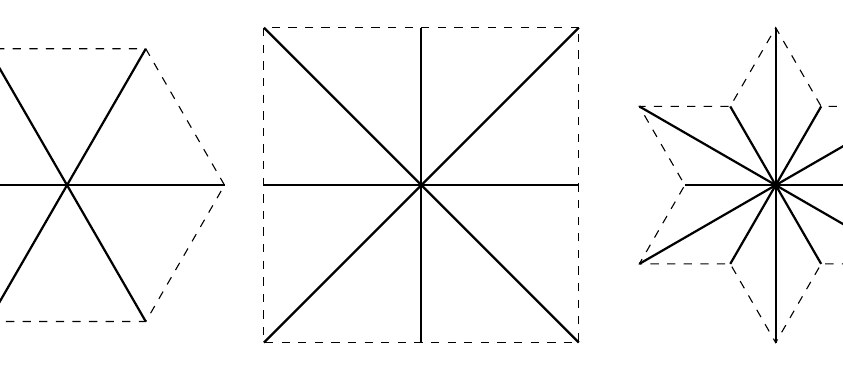
\begin{tikzpicture}
  \def\R{2.0}
  \def\rt3{1.732}
  \def\L{1.732} % R rt3 / 2
  \def\h{1/1.732} % R/( 2 rt3 )

  \useasboundingbox (-5,-2)  rectangle (5,2);

  % Define the coordinates
  \begin{scope}[shift={(-4.5,0)}]
    \coordinate (E) at (\R,0);
    \coordinate (NE) at (0.5*\R,\L);
    \coordinate (NW) at (-0.5*\R,\L);
    \coordinate (W) at (-\R,0);
    \coordinate (SW) at (-0.5*\R,-\L);
    \coordinate (SE) at (0.5*\R,-\L);
    %    -x   x        x = R/rt3
    %  W         E
    %    -x   x
    \draw[dashed] (E) -- (NE) -- (NW) -- (W) --  (SW) -- (SE) -- cycle;
    \draw[thick] (W)  -- (E) ;
    \draw[thick] (SW) -- (NE);
    \draw[thick] (NW) -- (SE);
  \end{scope}

  %\begin{scope}[shift={(0,0)}]
  \coordinate (E) at (\R,0);
  \coordinate (NE) at (\R,\R);
  \coordinate (N) at (0,\R);
  \coordinate (NW) at (-\R,\R);
  \coordinate (W) at (-\R,0);
  \coordinate (SW) at (-\R,-\R);
  \coordinate (S) at (0,-\R);
  \coordinate (SE) at (\R,-\R);

  \draw[dashed] (NE) -- (NW)-- (SW) -- (SE) -- cycle;
  \draw[thick] (W) -- (E);
  \draw[thick] (S) -- (N);
  \draw[thick] (SW) -- (NE);
  \draw[thick] (SE) -- (NW);

  %\end{scope}
  \begin{scope}[shift={(4.5,0)}]
    \coordinate (E) at (\R/\rt3,0);
    \coordinate (NE) at (\L,0.5*\R);
    \coordinate (NE2) at (\h,0.5*\R);
    \coordinate (N) at (0,\R);
    \coordinate (NW) at (-\L,0.5*\R);
    \coordinate (NW2) at (-\h,0.5*\R);
    \coordinate (W) at (-\R/\rt3,0);
    %      N      
    % -z'        z=(R/2,rt3 R/2), 
    %      +                     
    % -z        z' 
    %      S
    \coordinate (SW) at (-\L,-0.5*\R);
    \coordinate (SW2) at (-\h,-0.5*\R);
    \coordinate (S) at (0,-\R);
    \coordinate (SE) at (\L,-0.5*\R);
    \coordinate (SE2) at (\h,-0.5*\R);
    \coordinate (N) at (0,\R);

    \draw[dashed] (E) --  (NE) --  (NE2) -- (N) --  (NW2) --  (NW) -- (W) --  (SW) --  (SW2) -- (S) --  (SE2) --  (SE) -- cycle;

    \draw[thick] (W)  -- (E) ;
    \draw[thick] (SW2) -- (NE2);
    \draw[thick] (NW2) -- (SE2);
    \draw[thick] (S) -- (N);
    \draw[thick] (SW) -- (NE);
    \draw[thick] (NW) -- (SE);
  \end{scope}
\end{tikzpicture}

\subsection{The standard form of the infinitesimal group}
%\section{CLASSIFICATION OF THE SEMI-SIMPLE GROUPS}
%\subsection{The standard form of the infinitesimal group}
% ----->  page 16,  "In order to ... "
%\subsection{Properties of the roots}
%\subsection{The vector diagram}

\subsection{Properties of the roots}
\subsection{The vector diagram}
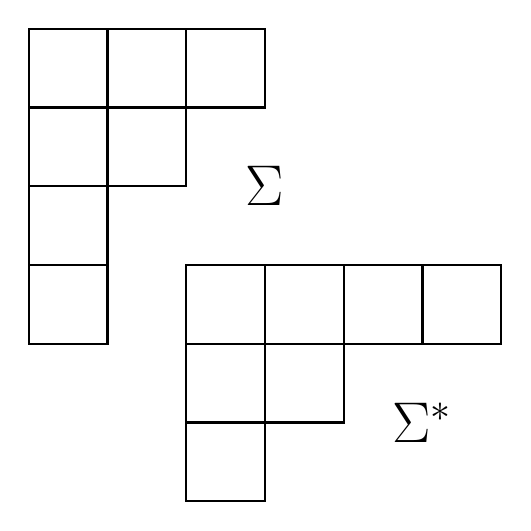
\begin{tikzpicture}
  \begin{scope}[shift={(-1,4)}]
    \foreach \x in {0,1,2} \draw[thick] (\x,0) rectangle (\x+1,-1);
    \foreach \x in {0,1}   \draw[thick] (\x,-1) rectangle (\x+1,-2);
    \foreach \x in {0}     \draw[thick] (\x,-2) rectangle (\x+1,-3);
    \foreach \x in {0}     \draw[thick] (\x,-3) rectangle (\x+1,-4);
    \node [font=\huge] at (3,-2) {$\Sigma$};
  \end{scope}
  \begin{scope}[shift={(1,1)}]
    \foreach \x in {0,1,2,3} \draw[thick] (\x,0) rectangle (\x+1,-1);
    \foreach \x in {0,1}   \draw[thick] (\x,-1) rectangle (\x+1,-2);
    \foreach \x in {0}       \draw[thick] (\x,-2) rectangle (\x+1,-3);
    \node [font=\huge] at (3,-2) {$\Sigma^{*}$};
  \end{scope}
\end{tikzpicture}



For Lecture 2, also see \cite{Weyl1926a,Weyl1926b, vanderWaerden1933, Coxeter1973}
and the article \cite[p.~186]{Weyl1934} by Coxeter.

The references for Lecture 3 are \cite{Cartan1913, Casimir1931, Casimir1935, Weyl1939, Racah1950a}.

The references for Lecture 4 are 
\cite{Condon1935, Weyl:1950:GTQ, Eckart1930, Wigner1931, vanderWaerden1974, Racah1942a, Racah1942b, Racah1943, Racah1949a, Wigner1941, Racah1949b, Jahn1950}

For Lecture 5 see \cite{Racah1950b}.
%Eugen Merzbacher (April 9, 1921 - June 6, 2013),
David Allen Park (1919 - January 19, 2012), 
Giulio Racah (February 9, 1909 - August 28, 1965).

\printbibliography[heading=bibintoc,title={References}]
\end{document}
